\documentclass{article}

\usepackage[letterpaper]{geometry}
\usepackage{amsmath}
\usepackage{amssymb}
\usepackage{siunitx}
\usepackage{graphicx}
\usepackage{tikz}

\title{4261 HW 5}
\author{Duncan Wilkie}
\date{?}

\begin{document}

\maketitle

\section*{1a}
This is a face-centered cubic lattice.

\section*{1b}
Taking the origin to be the lower-left atom, we take the basis vectors $[\frac{1}{2},\frac{1}{2},0]a$, $[\frac{1}{2},0,\frac{1}{2}]a$, $[0,\frac{1}{2},\frac{1}{2}]a$, where $a$ is the lattice constant.
The atoms in the conventional cell that aren't at one of these basis vectors may be readily constructed from them.

\section*{1c}
Looking at the fcc conventional cell, it is evident that adjacent Zn atoms are spaced by the distance from the center of the face to the corner; in terms of the lattice constant, this is
\[
  \ell=a/\sqrt{2}=(\SI{0.54}{nm})/\sqrt{2}=\SI{0.38}{nm}
\]
The S atoms will be spaced by the same amount, since their primitive unit cell is that of the Zn atoms translated by $[1/4,1/4,-1/4]a$.
The Zn-S spacing is the magnitude of this translation,
\[\sqrt{3a^{2}/16}=a\sqrt{3}/4=(\SI{0.54}{nm})\sqrt{3}/4=\SI{0.23}{nm}\]

\section*{1d}
\begin{center}
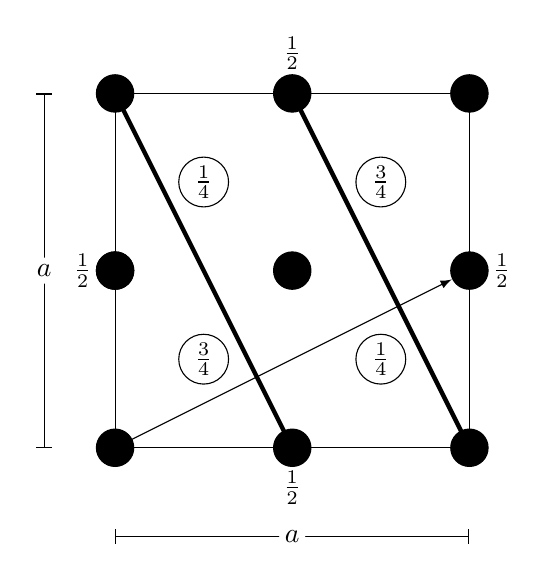
\begin{tikzpicture}[scale=4.5]
  \filldraw[black] (0,0) circle (1.5pt);
  \draw (0,0) -- (0.5,0);
  \filldraw[black] (0.5,0) circle (1.5pt) node[below,yshift=-5pt]{$\frac{1}{2}$};
  \draw (0.5,0) -- (1,0);
  \filldraw[black] (1,0) circle (1.5pt);
  \draw (1,0) -- (1,0.5);
  \filldraw[black] (1,0.5) circle (1.5pt) node[right,xshift=5pt]{$\frac{1}{2}$};
  \draw (1,0.5) -- (1,1);
  \filldraw[black] (1,1) circle (1.5pt);
  \draw (1,1) -- (0.5,1);
  \filldraw[black] (0.5,1) circle (1.5pt) node[above,yshift=5pt]{$\frac{1}{2}$};
  \draw (0.5,1) -- (0,1);
  \filldraw[black] (0,1) circle (1.5pt);
  \draw (0,1) -- (0,0.5);
  \filldraw[black] (0,0.5) circle (1.5pt) node[left,xshift=-5pt]{$\frac{1}{2}$};
  \draw (0,0.5) -- (0,0);
  \filldraw[black] (0,0.5) circle (1.5pt);

  \filldraw[black] (0.5,0.5) circle (1.5pt);

  \draw (0.25, 0.25) circle (2pt) node{$\frac{3}{4}$};
  \draw (0.25, 0.75) circle (2pt) node{$\frac{1}{4}$};
  \draw (0.75, 0.25) circle (2pt) node{$\frac{1}{4}$};
  \draw (0.75, 0.75) circle (2pt) node{$\frac{3}{4}$};


  \draw[|-|] (0,-0.25) -- (1,-0.25);
  \filldraw[white] (0.5,-0.25) circle (1pt);
  \node at (0.5,-0.25) (a) {$a$};

  \draw[|-|] (-0.2,0) -- (-0.2,1);
  \filldraw[white] (-0.2,0.5) circle (1pt);
  \node at (-0.2,0.5) (a) {$a$};

  \draw[-latex] (0,0) -- (0.95,0.475);


  \draw[ultra thick] (0,1) -- (0.5,0);
  \draw[ultra thick] (0.5,1) -- (1,0);

\end{tikzpicture}
\end{center}
Note that the arrow lies parallel to the $xy$-plane and the lattice planes are pointing out of the page from the lines representing them.

\section*{1e}
Notice from the image that the arrow representing the given direction has length $\sqrt{a^{2}+a^{2}/4}=a\sqrt{5}/2$, and along its length
there are two and a half instances of the lattice plane spacing. The spacing between planes is then $a\sqrt{5}/25$.

\section*{2}
A crystal plane is a plane overlaying a crystalline lattice that intersects at least three non-collinear points of the lattice.
Miller indices describe lattice planes by first constructing a reciprocal-space basis corresponding to a direct-space basis
of choice, and denoting points of the reciprocal lattice by $(hkl)$ where the numbers are the coefficients of the linear combination of
the reciprocal basis vectors that equals the point.
This represents a lattice plane by the one-to-one correspondence between reciprocal vectors and lattice planes normal to them.

The reciprocal lattice vector has components $b_{i}=2\pi/a_{i}$, and the family of lattice planes $(hkl)$ is normal to the reciprocal
lattice vector with components $h$, $k$, and $l$, so it will also be normal to the direct lattice vector $[hkl]$ since the relation
between the components is simply a constant multiplication.

% TODO: finish


\end{document}
%%% Local Variables:
%%% mode: latex
%%% TeX-master: t
%%% End:
